\documentclass{article}
\usepackage{mathtools, blkarray}
\usepackage{graphics,graphicx}
\usepackage{tikz}

\usetikzlibrary{arrows,snakes,backgrounds}



\makeatletter
% we use \prefix@<level> only if it is defined
\renewcommand{\@seccntformat}[1]{%
  \ifcsname prefix@#1\endcsname
    \csname prefix@#1\endcsname
  \else
    \csname the#1\endcsname\quad
  \fi}
% define \prefix@subsection
\newcommand\prefix@subsection{}
\makeatother

\makeatletter
% we use \prefix@<level> only if it is defined
\renewcommand{\@seccntformat}[1]{%
  \ifcsname prefix@#1\endcsname
    \csname prefix@#1\endcsname
  \else
    \csname the#1\endcsname\quad
  \fi}
% define \prefix@subsubsection
\newcommand\prefix@subsubsection{ }
\makeatother

\newcommand{\mytilde}{\raise.17ex\hbox{$\scriptstyle\mathtt{\sim}$}}


\begin{document}

\title{Math 775: Homework 3}
\author{Alex Dewey}


\maketitle

\section{Notes}

3.11. Start (bioassay is read though)

5.8. Proof is easy, must code/plot

Part II:

1. Start (coding is easy, theory a bit more careful)


\section{Exercises}

\subsection{Chapter 3 - Problem 8.}

Since our parameters \(y_i, z_i\) are in the form of proportions
and our data is binomial, it's natural to attempt to model this study 
using a beta-binomial model.

From the data, the average observed proportion of bikes is about 20\% for
blocks with a bike route  (\(y_i\)), with an average of 116 vehicles per block.
and blocks without a bike route have an average of around 10\% (\(z_i\)) bikes
and an average total of 87.375 vehicles per block.

There are a lot of vehicles and quite a lot of bikes, and we have little
background information. So the prior shouldn't matter too much in our inferences.

Therefore, let's use a relatively weak prior representing 20 total vehicles,
a certain fraction of which are bikes:
\(Beta(4, 16)\) for blocks with a bike route (so 4 bikes and 16 other vehicles) and 
\(Beta(2, 18)\) for blocks without. So we have four total parameters: 
\(\theta_y = (\alpha_y, \beta_y), \theta_z = (\alpha_z, \beta_z)\), two for each type of block.

With this prior, we'll next assume the sampling distribution for the parameters
is IID binomial for the 10 bike-route blocks and the 8 non-bike-route blocks,

For each block i, we let \(b_i, n_i\) be the number of bikes and total vehicles, respectively,
and add the data from the 10 + 8 blocks to each prior to produce their conjugate posterior.

So our posteriors will be \(Beta(\alpha_0 + \sum b_i,  \beta_0 + \sum (n_i - b_i))\) for both types
of blocks. This works out to
\(Beta(216, 964)\) for blocks with a bike route and
\(Beta(54, 665\) for blocks without.

Below are the histograms for 1000 sampled posterior means from each
block type's distribution \(\mu_y, \mu_z\), and
their difference \(\mu_y - \mu_z\).

\begin{figure}[!ht]
  \caption{The distribution of 
  \(y_i\) in n=1,000 posterior samples.}
  \centering
    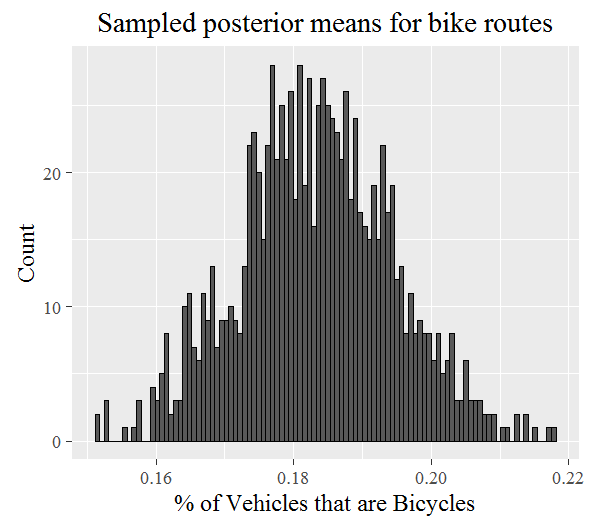
\includegraphics[width=\textwidth]{Problem38y}
\end{figure}    

\begin{figure}[!ht]
  \caption{The distribution of \(z_i\) in n=1,000 posterior samples.}
  \centering
    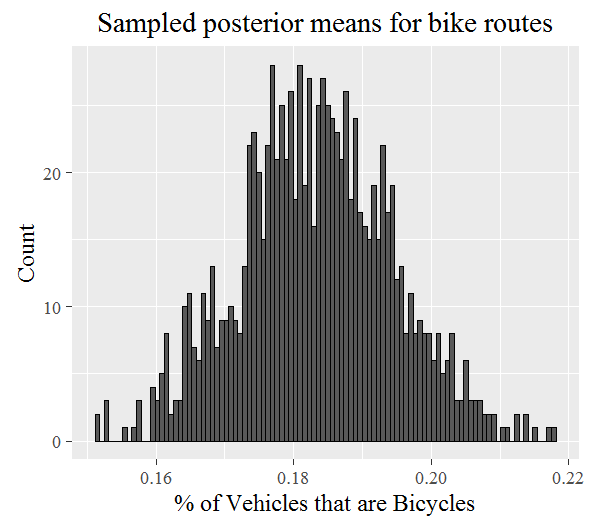
\includegraphics[width=\textwidth]{Problem38y}
\end{figure}    

\begin{figure}[!ht]
  \caption{The distribution of \(\mu_y - \mu_z\) in n=10,000 posterior samples.}
  \centering
    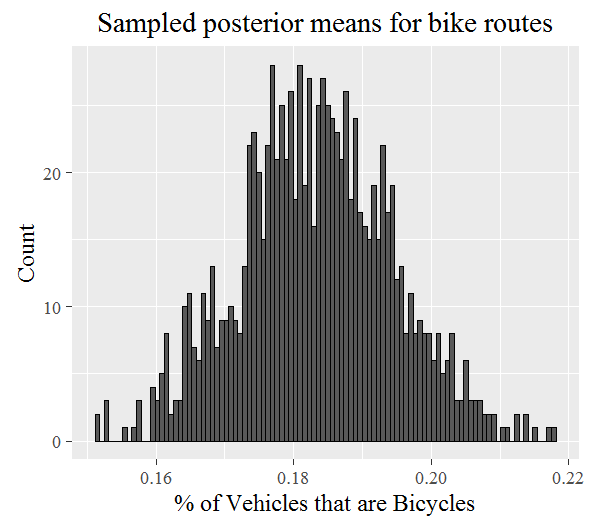
\includegraphics[width=\textwidth]{Problem38y}
\end{figure}    



\subsection{Chapter 3 - Problem 11.}

\subsection{Chapter 4 - Problem 2.}

\(p(\theta \vert y) \approx N(\hat{\theta}, [I(\hat{\theta})]^{-1})\).

where \(I(\theta) = -{d^2 \over d\theta^2}\log p(\theta \vert y)\).

We want to find \(I(\alpha, \beta)\), the observed information.
by the second derivatives (with respect to alpha and beta)
of the log posterior distribution. The likelihood is:

\[p(\alpha, \beta \vert y, n, x) \propto p(\alpha, \beta) 
\prod p(y_i \vert \alpha, \beta, n_i, x_i),\]
where \(p(\alpha, \beta) \propto 1,\) and the sampling distribution.
\[p(y_i \vert \alpha, \beta, n_i, x_i) \propto [f(\alpha + \beta x_i)]^{y_i}
[1 - f(\alpha + \beta x_i)]^{n_i - y_i}\], where \(f(x) = logit^{-1}(x)\), the
inverse-logit function (or the logistic function).

So the log posterior is
\[\log p(\alpha, \beta \vert y, n, x) = 
C + \sum \log p(y_i \vert \alpha, \beta, n_i, x_i) =\]
\[C +  \sum \log \big[ [f(\alpha + \beta x_i)]^{y_i}
[1 - f(\alpha + \beta x_i)]^{n_i - y_i}\big] = \].
\[ C + \sum y_i \log f(\alpha + \beta x_i) +
(n_i - y_i)\log (1 - f(\alpha + \beta x_i))\].

The definition of 
and derivative of the inverse-logit (aka the logistic function) are
(per Wikipedia):

\(f(x) = {e^x \over e^x + 1}\) and \({d \over dx} f(x) = f(x)\times (1 - f(x))\).

So \({d \over dx} \log f(x) = {f'(x)\over f(x)} = 1 - f(x) \).

So the first derivatives of the log posterior are:
\[{d \log p(\alpha, \beta \vert y, n, x) \over d\alpha} = 
\sum y_i {f'(\alpha + \beta x_i) \over f(\alpha + \beta x_i)} -
(n_i - y_i){f'(\alpha + \beta x_i) \over 1 - f(\alpha + \beta x_i)} = \]
\[\sum y_i (1 - f(\alpha + \beta x_i)) -
(n_i - y_i)f(\alpha + \beta x_i) =
\sum y_i - n_i f(\alpha + \beta x_i)\]
and:
\[{d \log p(\alpha, \beta \vert y, n, x) \over d\beta} = 
\sum x_i y_i {f'(\alpha + \beta x_i) \over f(\alpha + \beta x_i)} -
x_i (n_i - y_i){f'(\alpha + \beta x_i) \over 1 - f(\alpha + \beta x_i)} = \]
\[\sum x_i y_i (1 - f(\alpha + \beta x_i)) -
x_i (n_i - y_i)f(\alpha + \beta x_i) =
\sum x_i (y_i - n_i f(\alpha + \beta x_i))\]

Setting these first derivatives to 0 yields the familiar normal equations 
from linear regression. The posterior mode, then, is the MLE
for \(\alpha, \beta\), i.e. the line of best fit on a logistic regression with predictors \(x_i\), 
response \(y_i\), and weights \(n_i\).

Gelman (p. 76) samples \((\hat{\alpha}, \hat{\beta}) \approx (0.8, 7.7)\)
as the posterior mode for this problem. I did the logistic regression in 
R to get (0.847, 7.749), which should be fine since we're already
trying to get a normal approximation.

Anyway, the second derivatives are:

\[{d^2 \log p(\alpha, \beta \vert y, n, x) \over d\alpha^2} = 
-\sum n_i f(\alpha + \beta x_i) (1 - f(\alpha + \beta x_i))\]

\[{d^2 \log p(\alpha, \beta \vert y, n, x) \over d\alpha d\beta} = 
-\sum x_i n_i f(\alpha + \beta x_i) (1 - f(\alpha + \beta x_i))\]

\[{d^2 \log p(\alpha, \beta \vert y, n, x) \over d\beta^2} = 
-\sum x_i^2 n_i f(\alpha + \beta x_i) (1 - f(\alpha + \beta x_i)) \].

For simplicity, define:
\(p_i = f(\alpha + \beta x_i)\) and \(q_i = 1 - p_i\). Then the information matrix is just:

\( I(\alpha, \beta) = 
\begin{bmatrix*}
  \sum n_i p_i q_i & \sum x_i n_i p_i q_i  \\
\sum x_i n_i p_i q_i & \sum x_i^2 n_i p_i q_i \\
 \end{bmatrix*}
\)

Using R, we can compute:

At our posterior mode, \((\hat{\alpha}, \hat{\beta}) \approx (0.847, 7.749)\),
this evaluates to:

\( I(\hat{\alpha}, \hat{\beta}) \approx
\begin{bmatrix*}
  1.965 & -0.293  \\
  -0.293 & 0.0859 \\
 \end{bmatrix*}
\)

Its inverse is
\( I^{-1}(\hat{\alpha}, \hat{\beta}) \approx
\begin{bmatrix*}
  0.509 & -3.408 \\
 -3.408 & 11.636 \\
 \end{bmatrix*}
\).

So the normal approximation is

\( p(\hat{\alpha}, \hat{\beta} \vert y, n, x) \approx
N \big( 
 \begin{pmatrix*}
0.847 \\
7.749 \\
 \end{pmatrix*}, 
\begin{pmatrix*}
  0.509 & -3.408 \\
 -3.408 & 11.636 \\
 \end{pmatrix*}
 \big)
\)



\subsection{Chapter 5 - Problem 1.}

\subsubsection{a.} 
\paragraph{Exchangeable?} Yes, all outcomes are equiprobable and therefore trivially exchangeable
\paragraph{Independent?} Yes, the two draws are IID.

\subsubsection{b.} 
\paragraph{Exchangeable?} Yes, there are only two outcomes (BW, WB) but they are equiprobable and
so they are exchangeable. 
\paragraph{Independent?} No, these outcomes are obviously not independent. The first draw determines the second draw.
\paragraph{Can we act as if the outcomes are independent?} No, because the first draw contains all the information
needed to determine the second draw. Probability is a measure of uncertainty and knowing the first outcome
removes all randomness from the second outcome. It wouldn't make sense to treat the information gained
from the second draw as independent from that of the first.

\subsubsection{c.}

\paragraph{Exchangeable?} Yes, there are only two outcomes for which
exchangeability is even relevant (BW, WB), and they are equiprobable and hence exchangeable. 
\paragraph{Independent?} No. There is a slight dependency between the two draws. Drawing
white first means that there are now 999,999 white balls and one million black balls left,
so the next draw is slightly weighted towards black.
\paragraph{Can we act as if the outcomes are independent?} Yes, assuming we don't
need accuracy in this experiment out to 6 or 7 places. While the first draw does slightly reduces the uncertainty 
in the second draw, it's a very small difference indeed.

\subsection{Chapter 5 - Problem 4.}

\subsubsection{a.} 
The observed data are exchangeable: Knowing only a priori that there are exactly J draws from one
distribution with mean 1and J draws from the other distribution with mean -1, every permutation is as likely as any other.

If we knew which draws were taken from each distribution, then this would no longer be true--if, for example, we consider the simple case with \(2J = 2\), where we have one draw from \(N(1,1)\) and one from \(N(-1,1\), then, in expectation, the result of the first draw would reduce our uncertainty about the second draw's distribution.

\subsection{b.}
Suppose this distribution could be written as the sum of IID components. Then take 2J to be a very large number. By the Central Limit Theorem, this should eventually look like a normal distribution around the mean 0 with variance \(1/2J\)--but instead, we have a bimodal distribution with two separate normal probability clusters around 1 and -1 with variance \(1/J\). So our assumption that this distribution can be written as the sum of IID components must be false.

\subsection{c.}

As J goes to infinity this becomes a hierarchical model with an implicit two-step sampling procedure--
for each \(\theta_i\), we first draw \(y_i = -1,1\) from the population distribution (a Bernoulli with hyperparameter 0.5), then
we actually draw \(\theta_i \vert y_i \mytilde N(y_i, 1)\). The trouble with applying De Finetti's Theorem
is that while the \(y_i\) \textit{are} clearly exchangeable, the \(\theta_i, \theta_j \vert y_i, y_j\) are no longer exchangeable 
even pairwise if \(y_i \neq y_j\), because we know that the two draws come from different distributions.

\subsection{Chapter 5 - Problem 5.}

The \(\theta_i\) are conditionally-IID on \(\phi\). 

Ignoring all the other \(\theta_i\), without loss of generality
let \(i = 1, j = 2\) and consider \(cov(\theta_1, \theta_2)\)

\(p(\theta_1, \theta_2) = \int p(\theta_1 \vert \phi) p(\theta_2 \vert \phi) p(\phi) d\phi = p(\theta_2, \theta_1)\).

So \(\theta_i\) is exchangeable. Let \(\bar{\theta}\) be the common mean of each \(\theta_i\).

\[cov(\theta_1, \theta_2) = E[(\theta_1 - \bar{\theta})(\theta_2 - \bar{\theta})] = \]
\[E[\theta_1\theta_2] - \bar{\theta}E[\theta_1 + \theta_2] + \bar{\theta}^2 = 
E[\theta_1\theta_2] - E[\theta_1]^2.\] Now,

\[E[\theta_1\theta_2]  = \int \int \int \theta_1 \theta_2 p(\theta_1 \vert \phi) p(\theta_2 \vert \phi) p(\phi)  d\theta_2 d\theta_1 d\phi. \]

\[E[\theta_1\theta_2]  = \int  p(\phi) \int \theta_1 p(\theta_1 \vert \phi)d \theta_1  \int \theta_2 p(\theta_2 \vert \phi) d\theta_2 d\phi. \]

\[E[\theta_1\theta_2]  = \int  p(\phi) \bigg[ \int \theta_1 p(\theta_1 \vert \phi) d\theta_1\bigg]^2  d\phi.\]
\[E[\theta_1\theta_2]  = \int  p(\phi) E[\theta_1 \vert \phi]^2  d\phi 
= E_{\phi} [E[\theta_1 \vert \phi]^2] \geq E_{\phi}[E[\theta_1 \vert \phi]]^2 = \]
\[\big[ \int  p(\phi) E[\theta_1 \vert \phi] d\phi\big]^2 = E[\theta_1]^2.\]

So \[cov(\theta_1, \theta_2) = E[\theta_1\theta_2] - E[\theta_1]^2 \geq 0.\]




\subsection{Chapter 5 - Problem 8.}


Show that the posterior can be written as the sum of the individual posteriors.

\subsection{Part 2 - Problem 1}



\end{document}